% --------------------------------------------------------------
%                         Preamble
% --------------------------------------------------------------

\documentclass[12pt, letter]{article}
\usepackage[latin1]{inputenc}
\usepackage[T1]{fontenc}
\usepackage{amsmath,amssymb,amsthm}
\usepackage{longtable}
\usepackage{enumitem}
\usepackage{hyperref}
\usepackage{verbatim}
\usepackage{bm}
\usepackage[framemethod=tikz]{mdframed}
\usepackage{graphicx}
\usepackage{amsmath}
\hypersetup{
    colorlinks=true,
    linkcolor=blue,
    filecolor=magenta,      
    urlcolor=blue,
}
 
\urlstyle{same}

\usepackage{array}
\newcolumntype{L}[1]{>{\raggedright\let\newline\\\arraybackslash\hspace{0pt}}m{#1}}
\newcolumntype{C}[1]{>{\centering\let\newline\\\arraybackslash\hspace{0pt}}m{#1}}
\newcolumntype{R}[1]{>{\raggedleft\let\newline\\\arraybackslash\hspace{0pt}}m{#1}}
\newcommand{\norm}[1]{\left\lVert#1\right\rVert}
\newcommand{\vs}[1][1]{\vspace{#1\baselineskip}}

\DeclareMathOperator{\depth}{depth}
\DeclareMathOperator{\im}{im}
\DeclareMathOperator{\coker}{coker}
\DeclareMathOperator{\rank}{rank}
\DeclareMathOperator{\Proj}{Proj}
\DeclareMathOperator{\Hom}{Hom}
\DeclareMathOperator{\Tor}{Tor}
\DeclareMathOperator{\Ext}{Ext}
\DeclareMathOperator{\HH}{H}

% page format

\topmargin -15mm \textwidth 168mm \textheight 240mm \oddsidemargin
-8mm \evensidemargin 0mm
\setlength{\parindent}{0pt}

% some environments :

\theoremstyle{plain}
\newtheorem{theorem}{Theorem}
\newtheorem{lemma}[theorem]{Lemma}
\newtheorem{corollary}[theorem]{Corollary}
\newtheorem{proposition}[theorem]{Proposition}

\numberwithin{theorem}{section}

\theoremstyle{definition}
\newtheorem{definition}[theorem]{Definition}
\newtheorem{example}[theorem]{Example}
\newtheorem{problem}[theorem]{Problem}
\newtheorem{exercise}[theorem]{Exercise}
\newtheorem{algorithm}[theorem]{Algorithm}
\newtheorem{note}[theorem]{Note}
\newtheorem{remark}[theorem]{Remark}
\newtheorem{question}[theorem]{Question}

% using AMS mathematical symbols

\usepackage{latexsym}            % for the qed symbol
\usepackage{amssymb}

\newcommand{\N}{\mathbb{N}}
\newcommand{\Z}{\mathbb{Z}}
\newcommand{\Q}{\mathbb{Q}}
\newcommand{\R}{\mathbb{R}}

\def\qex{\hfill \quad\vrule height1.2ex width0.5em depth 0pt} % end of example


\begin{document}

% --------------------------------------------------------------
%                         Start here
% --------------------------------------------------------------

\noindent
Colorado State University \hfill Section 5 (4:00-4:50pm)\\
Department of Mathematics\ \  \hfill  Math 261, Fall 2019\\
\bigskip
\thispagestyle{empty}

\begin{center}
\begin{large}
\textbf{Lecture Notes-Midterm 3\\
}
\end{large}
\end{center}

% --------------------------------------------------------------
%                         Intro
% --------------------------------------------------------------

\noindent These notes were created by Scott Ziegler for Math 261 at Colorado State University and adapted from Thomas' Calculus, 13th Edition, Pearson Education Inc, 2010. The listed section numbers correspond to the sections of the aforementioned text.


% --------------------------------------------------------------
%                         Sec 15.1
% --------------------------------------------------------------

\section{Double and Iterated Integrals over Rectangles (15.1)}

The concept of an integral of a function of one variable should be very clear to us by now. As we move to discussing integrals of functions of multiple variables our intuition will come from integrals of functions of one variable. However, instead of integrating over an interval of the x-axis we are now integrating over a region of space.

\bigskip

We'll start talking about integrals by considering what happens when the region of space is a rectangle. Let $f(x,y)$ be a function defined on the rectangular region $R: \ a \leq x \leq b, \ c \leq y \leq d$. We'll subdivide $R$ into $n$ rectangular pieces as follows:

\bigskip

\begin{center}
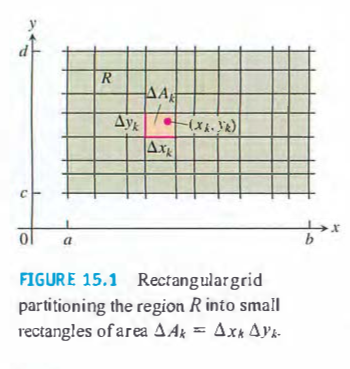
\includegraphics[scale=0.7]{m3_f1}
\end{center}

\bigskip

Now let the rectangles have the width $\Delta x_k$ and height $\Delta y_k$, then each of these rectangles has area $\Delta A_k = \Delta x_k \Delta y_k$. Now pick a point $(x_k,y_k)$ in the $k^{\text{th}}$ rectangle. Then the value $f(x_k,y_k) \delta A_k$ approximates the volume of a small portion of the full volume under $f(x,y)$ in the region $R$. If we sum up all of these volumes we get
\begin{align*}
\sum_{k=1}^n f(x_k,y_k) \Delta A_k.
\end{align*}
This should look very much like the Riemann sums we saw in Calc I! Now as I take the number of rectangles $n$ to infinity I get
\begin{align*}
\lim_{n\to\infty} \sum_{k=1}^n f(x_k,y_k) \Delta A_k.
\end{align*}
When this limit exists the function $f$ is said to be $\textbf{integrable}$ and limit is called the integral of $f$ over $R$.
\begin{align*}
\int \int_R f(x,y) dA = \int \int_{R} f(x,y) dx dy = \lim_{n\to\infty} \sum_{k=1}^n f(x_k,y_k) \Delta A_k.
\end{align*}

\bigskip

\hrulefill

\bigskip

Suppose we want to find the volume under the plane $z=4-x-y$ over the rectangular region $R: \ 0 \leq x \leq 2, 0 \leq y \leq 1$. We could use the method of cross sections from Calc I to state that the volume is
\begin{align*}
V = \int_{x=0}^{x=2} A(x) dx
\end{align*}
where $A$ is the cross-sectional area at $x$.

\bigskip

\begin{center}
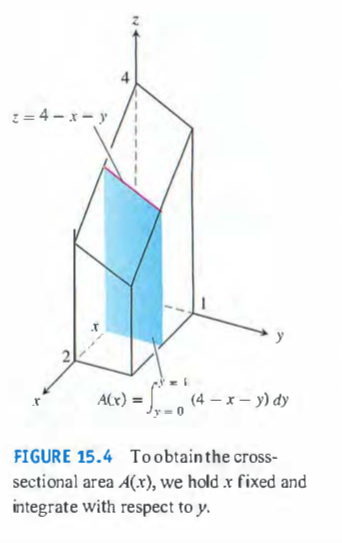
\includegraphics[scale=0.7]{m3_f2}
\end{center}

\bigskip

This cross-sectional area can be found by holding $x$ fixed in $z=4-x-y$ and integrating with respect to $y$ (finding the area under the $y$-axis). Thus
\begin{align*}
A(x) = \int_{y=0}^{y=1} (4-x-y) dy.
\end{align*}
So now our volume is
\begin{align*}
V &= \int_{x=0}^{x=2} A(x) dx\\
&= \int_{x=0}^{x=2} \left(\int_{y=0}^{y=1} (4-x-y)dy \right) dx\\
&= \int_{x=0}^{x=2} \left[ 4y-xy-\frac{y^2}{2}\right]_{y=0}^{y=1} dx\\
&= \int_{x=0}^{x=2} \left(\frac{7}{2} - x\right)dx\\
&= \left[ \frac{7}{2}x-\frac{x^2}{2} \right]_{x=0}^{x=2}\\
&=5.
\end{align*}

\bigskip

But what if we had instead found the volume by ``cutting" in the other direction? That is, what if we had found
\begin{align*}
V = \int_{y=0}^{y=1} A(y)dy
\end{align*}
where $A$ is the cross-sectional area at $y$?

\bigskip

\begin{center}
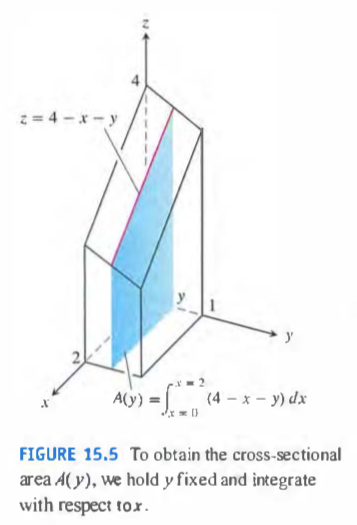
\includegraphics[scale=0.7]{m3_f3}
\end{center}

\bigskip

This cross-sectional area can be found by holding $y$ fixed in $z=4-x-y$ and integrating with respect to $x$ (finding the area under the $x$-axis). Thus
\begin{align*}
A(y) = \int_{x=0}^{x=2} (4-x-y) dx.
\end{align*}
So now our volume is
\begin{align*}
V &= \int_{y=0}^{y=1} A(y) dy\\
&= \int_{y=0}^{y=1} \left(\int_{x=0}^{x=2} (4-x-y)dx \right) dy\\
&= \int_{y=0}^{y=1} \left[ 4x-\frac{x^2}{2}-xy\right]_{x=0}^{x=2} dy\\
&= \int_{y=0}^{y=1} \left(6-2y\right)dy\\
&= \left[ 6y-y^2 \right]_{y=0}^{y=1}\\
&=5.
\end{align*}

\bigskip

This leads to the following.

\bigskip

\begin{theorem}{(Fubini's Theorem)}
\\
If $f(x,y)$ is continuous throughout the rectangular region $R: \ a\leq x\leq b, \ c\leq y\leq d$, then
\begin{align*}
\int \int_R f(x,y) dA = \int_c^d \int_a^b f(x,y)dx dy = \int_a^b \int_c^d f(x,y)dydx.
\end{align*}
\end{theorem}

\bigskip

The terms $\int_c^d \int_a^b f(x,y)dx dy$ and  $\int_a^b \int_c^d f(x,y)dydx$ are called \textbf{iterated integrals}. This theorem says not only can double integrals be calculated as iterated integrals, but that it doesn't matter which order we do the integrals in.

\bigskip

\hrulefill

\bigskip

\begin{example}
Calculate $\int \int_R f(x,y) dA$ for
\begin{align*}
f(x,y) = 100-6x^2y \ \ \text{and} \ \ R: \ 0\leq x \leq 2, \ -1 \leq y \leq 1.
\end{align*}

\bigskip

Here we have
\begin{align*}
\int \int_R f(x,y) dA &= \int_{-1}^1 \int_0^2 (100-6x^2y)dxdy\\
&= \int_{-1}^1 \left[100x-2x^3y\right]_{x=0}^{x=2} dy\\
&= \int_{-1}^1 (200-16y)dy\\
&=\left[200y-8y^2\right]_{-1}^1\\
&=400.
\end{align*}
We also could have integrated with respect to $y$ first!
\end{example}

\bigskip

\hrulefill

\bigskip

\begin{example}
Find the volume of the region bounded above by the elliptical paraboloid $z=10+x^2+3y^2$ and below by the rectangle $R: \ 0\leq x \leq 1, \ 0\leq y \leq 2$.

\bigskip

Here we have
\begin{align*}
V= \int \int_R (10+x^2+3y^2) dA 
&= \int_0^1 \int_0^2 (10+x^2+3y^2)dydx\\
&= \int_0^1 \left[10y+x^2y+y^3\right]_{y=0}^{y=2} dx\\
&= \int_0^1 (20+2x^2+8)dx\\
&=\left[20x+\frac{2}{3}x^3+8x\right]_0^1\\
&=\frac{86}{3}.
\end{align*}
We also could have integrated with respect to $y$ first!
\end{example}

\newpage

% --------------------------------------------------------------
%                         Sec 15.2
% --------------------------------------------------------------

\section{Double Integrals over Bounded Regions (15.2)}

Now we will see how to evaluate double integrals when the region in question is no longer a rectangle.

\bigskip

The process here proceeds exactly as it did in the last section. If our region looks like the following 

\bigskip

\begin{center}
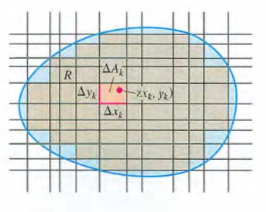
\includegraphics[scale=0.7]{m3_f8}
\end{center}

\bigskip

then we form a partition of $R$ by breaking the region up into rectangles. Notice now however that the rectangles don't nicely fill the region! That's okay however, as we make the rectangles small we won't have to worry about that for most regions. The volume under the curve and above $R$ is approximated by
\begin{align*}
S_n = \sum_{k=1}^n f(x_k,y_k) \Delta A_k
\end{align*}
and as we make the rectangles small we again get
\begin{align*}
\lim_{n\to\infty} \sum_{k=1}^n f(x_k,y_k)\Delta A_k = \int \int_R f(x,y) dA.
\end{align*}

The only difference here is that the bounds on the integral will no longer be constants for both $x$ and $y$!

\bigskip

\hrulefill

\bigskip

Say our region $R$ in the $xy$-plane is bounded on the sides by the lines $x=a$ and $x=b$, and above and below by the curves $y=g_2(x)$ and $y=g_1(x)$. (Draw a picture of this region). We can find the volume by using cross sections. Finding the cross sectional area here gives
\begin{align*}
A(x) = \int_{y=g_1(x)}^{g_2(x)} f(x,y)dy.
\end{align*}
(Discuss this by visualizing a curve coming out of the board. We fix $x$ and integrate over $y$ to get one of the cross sections!). Now we integrate this cross sectional area from $x=a$ to $x=b$ to get the volume
\begin{align*}
V=\int_a^b A(x)dx = \int_a^b \int_{y=g_1(x)}^{y=g_2(x)} f(x,y)dy dx.
\end{align*}

\bigskip

If $R$ is instead the region bounded on the sides by the curves $x=h_2(y)$ and $x=h_1(y)$ and above and below by the lines $y=c$ and $y=d$ (draw a picture of this region) we would get
\begin{align*}
V=\int_c^d A(y)dy = \int_c^d \int_{x=h_1(y)}^{x=h_2(y)} f(x,y)dxdy.
\end{align*}

\bigskip

\hrulefill

\bigskip

\begin{theorem}{(Fubini's Theorem)}
\\
Let $f(x,y)$ be continuous on a region $R$.
\begin{itemize}
\item[1.] If $R$ is defined on $a\leq x\leq b$, $g_1(x)\leq y \leq g_2(x)$, with $g_1$ and $g_2$ continuous on $[a,b]$, then
\begin{align*}
\int \int_R f(x,y)dA = \int_a^b \int_{g_1(x)}^{g_2(x)} f(x,y)dydx.
\end{align*}
\item[2.]If $R$ is defined on $c\leq y\leq d$, $h_1(y)\leq x \leq h_2(y)$, with $h_1$ and $h_2$ continuous on $[c,d]$, then
\begin{align*}
\int \int_R f(x,y)dA = \int_c^d \int_{h_1(y)}^{h_2(y)} f(x,y)dxdy.
\end{align*}
\end{itemize}
\end{theorem}

\bigskip

\hrulefill

\bigskip

The only change in computing these integrals as compared to the last section is that we need to start by finding the region of integration! To do this, follow these steps.

\begin{itemize}
\item[1.] Sketch the region of integration and label the bounding curves.
\item[2.] If using vertical cross sections, draw a vertical line through the region and set the $y$-values equal to where the line enters and leaves the region. If using horizontal cross sections, draw a horizontal line through the region and set the $x$-values equal to where the line enters and leaves the region.
\item[3.] If using vertical cross sections, choose $x$-values that will include all vertical lines through the region. If using horizontal cross sections, choose $y$-values that will include all horizontal lines through the region.
\end{itemize}

\bigskip

\hrulefill

\bigskip

\begin{example}
Sketch the region of integration for the integral
\begin{align*}
\int_0^2 \int_{x^2}^{2x} (4x+2) dy dx
\end{align*}
and write an equivalent integral with the order of integration reversed.

\bigskip

Our $y$ values encompass the interval $x^2\leq y \leq 2x$ when $0\leq x \leq 2$. Therefore our region looks like this.

\bigskip

\begin{center}
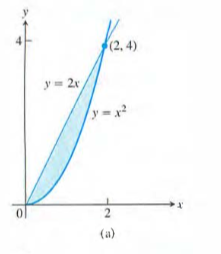
\includegraphics[scale=0.7]{m3_f4}
\end{center}

\bigskip

If we instead wanted to integrate with respect to $x$ first and then $y$ we would draw a horizontal line through our regions and consider what curve is on the right of that line and which is on the left. We see that the curve $y=x^2 \Rightarrow x=\sqrt{y}$ is on the right and $y=2x \Rightarrow x=\frac{y}{2}$ is on the left. We can also see that the $y$ values in this region run from $0$ to $4$. Therefore our integral with the order of integration reversed is
\begin{align*}
\int_0^4 \int_{y/2}^{\sqrt{y}} (4x+2)dxdy.
\end{align*}

\end{example}

\bigskip

\hrulefill

\bigskip

\begin{example}
Find the volume of the prism whose base is the triangle in the $xy$-plane bounded by the $x$-axis and the lines $y=x$ and $x=1$ and whose top lies in the plane
\begin{align*}
z=f(x,y) = 3-x-y.
\end{align*}

\bigskip

We first need to find the limits of integration, so we will begin by making a sketch of the region.

\bigskip

\begin{center}
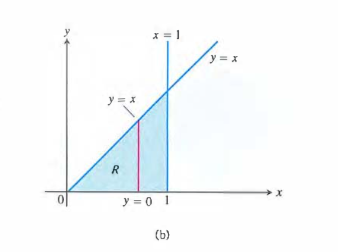
\includegraphics[scale=0.7]{m3_f5}
\end{center}

\bigskip

If we first want to integrate with respect to $y$ we can use the above drawing to see our volume is
\begin{align*}
V&=\int_0^1 \int_0^x (3-x-y)dydx\\
&=\int_0^1 \left[3y-xy-\frac{y^2}{2}\right]_{y=0}^{y=x} dx\\
&= \int_0^1 \left(3x-\frac{3}{2}x^2\right)dx\\
&=\left[\frac{3}{2}x^2-\frac{x^3}{2}\right]_0^1\\
&=1.
\end{align*}

Now if we want to find the volume by instead integrating with respect to $x$ first we can use the following picture

\bigskip

\begin{center}
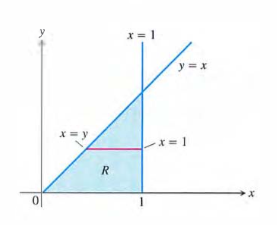
\includegraphics[scale=0.7]{m3_f6}
\end{center}

\bigskip

to see that our volume is
\begin{align*}
V&=\int_0^1 \int_y^1 (3-x-y)dxdy\\
&=\int_0^1 \left[3x-\frac{x^2}{2}-xy\right]_{x=y}^{x=1}dy\\
&= \int_0^1 \left(3-\frac{1}{2}-y-3y+\frac{y^2}{2}+y^2\right)dy\\
&= \int_0^1 \left(\frac{5}{2}-4y+\frac{3}{2}y^2\right)dy\\
&= \left[\frac{5}{2}y-2y^2+\frac{y^3}{2}\right]_0^1\\
&=1.
\end{align*}

\end{example}

\bigskip

\hrulefill

\bigskip

While Fubini's Theorem tells us we \textit{can} do the double integral in either way and get the same answer, it is sometimes much easier to do the integral with respect to one of the variables first!

\bigskip

\hrulefill

\bigskip

\begin{example}
Calculate 
\begin{align*}
\int \int_R \frac{\sin(x)}{x}dA,
\end{align*}
where $R$ is the triangle in the $xy$-plane bounded by the $x$-axis, the line $y=x$, and the line $x=1$.

\bigskip

Our region here looks like this:

\bigskip

\begin{center}
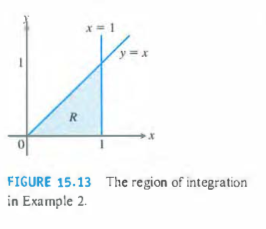
\includegraphics[scale=0.7]{m3_f7}
\end{center}

\bigskip

If we want to integrate with respect to $y$ first, our integral is
\begin{align*}
\int_0^1 \int_0^x \frac{\sin(x)}{x} dy dx &= \int_0^1 \left[y\frac{\sin(x)}{x}\right]_{y=0}^{y=x} dx\\
&=\int_0^1 \sin(x)dx\\
&=-\cos(1)+1.
\end{align*}
But if we try to integrate with respect to $x$ first we get
\begin{align*}
\int_0^1 \int_y^1 \frac{\sin(x)}{x}dxdy,
\end{align*}
which we cannot compute by hand!

\end{example}

\newpage

% --------------------------------------------------------------
%                         Sec 15.3
% --------------------------------------------------------------

\section{Areas by Double Integration (15.3)}

Looking back at our Riemann sum we used to find double integrals, note that letting $f(x,y)=1$ gives
\begin{align*}
S_n &= \sum_{k=1}^n f(x_k,y_k)\Delta A_k\\
&= \sum_{k=1}^n \Delta A_k.
\end{align*}
This is the sum of all the small rectangles used to partition $R$. So if we let $n \to \infty$, we will get the exact area inside of $R$.

\bigskip

\begin{definition}
The \textbf{area} of a closed, bounded plane region $R$ is
\begin{align*}
A = \int \int_R dA.
\end{align*}
\end{definition}

\bigskip

\hrulefill

\bigskip

\begin{example}
Find the area of the region $R$ bounded by $y=x$ and $y=x^2$ in the first quadrant.

\bigskip

We should make a sketch of the region.

\bigskip

\begin{center}
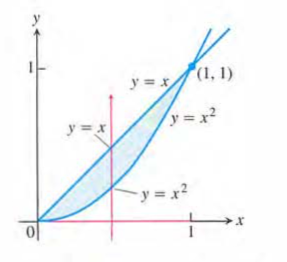
\includegraphics[scale=0.7]{m3_f9}
\end{center}

\bigskip

Using this we can set up our integral as
\begin{align*}
A &= \int_0^1 \int_{x^2}^x dy dx\\
&= \int_0^1 \left[ y\right]_{x^2}^x dx\\
&= \int_0^1 (x-x^2)dx\\
&= \left[ \frac{x^2}{2} - \frac{x^3}{3} \right]_0^1\\
&= \frac{1}{6}.
\end{align*}

\end{example}

\bigskip

\hrulefill

\bigskip

\begin{example}
Find the area of the region $R$ enclosed by the parabola $y=x^2$ and the line $y=x+2$.

\bigskip

Our area here looks like this.

\bigskip

\begin{center}
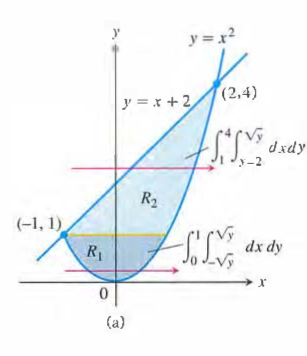
\includegraphics[scale=0.7]{m3_f10}
\end{center}

\bigskip

Remember, we can set up our integral by integrating with respect to either $x$ or $y$ first. But in this case one of the directions is easier.

\smallskip

Breaking the region into $R_1$ and $R_2$ like the figure above gives
\begin{align*}
A &= \int \int_{R_1} dA + \int \int_{R_2} dA\\
&= \int_0^1 \int_{-\sqrt{y}}^{\sqrt{y}} dxdy + \int_1^4 \int_{y-2}^{\sqrt{y}} dx dy.
\end{align*}
But if we instead integrate with respect to $y$ first we get
\begin{align*}
A &= \int_{-1}^2 \int_{x^2}^{x+2} dy dx\\
&= \int_{-1}^2 (x+2-x^2)dx\\
&=\left[\frac{x^2}{2}+2x-\frac{x^3}{3}\right]_{-1}^3\\
&= \frac{9}{2}.
\end{align*}

\end{example}

\bigskip

\hrulefill

\bigskip

Recall that for a function of one variable the average value of the function over an interval was the integral of the function over that interval divided by the length of the interval. That should make the next definition pretty believable.

\begin{definition}
The \textbf{average value} of $f$ over $R$ is
\begin{align*}
\frac{1}{\text{area of } R} \int \int_R fdA.
\end{align*}
\end{definition}

\bigskip

\hrulefill

\bigskip

\begin{example}
Find the average value of $f(x,y) = x\cos(xy)$ over the rectangle $R: \ 0\leq x \leq \pi, \ 0\leq y \leq 1$.

\bigskip

The average value $A_f$ is
\begin{align*}
A_f&=\frac{1}{\text{area}(R)} \int_0^\pi \int_0^1 x\cos(xy) dydx\\
&= \frac{1}{\pi} \int_0^\pi \left[\sin(xy)\right]_{y=0}^{y=1} dx\\
&= \frac{1}{\pi} \int_0^\pi \sin(x)dx\\
&= \frac{1}{\pi} \left[-\cos(x)\right]_0^\pi\\
&= \frac{2}{\pi}.
\end{align*}
\end{example}

\newpage

% --------------------------------------------------------------
%                         Sec 15.4
% --------------------------------------------------------------

\section{Double Integrals in Polar Form (15.4)}

Recall polar coordinates from Calc II. Polar coordinates are just a different way to draw grid lines in 2 dimensions compared to cartesian coordinates. Instead of drawing rectangles parallel to the $x$ and $y$ axes, we draw our grid lines with respect to the radial distance from the origin and the angle with respect to the $x$-axis. Let's do a quick example to refresh our memory.

\bigskip

\hrulefill

\bigskip

\begin{example}
Graph the curve $r=1+\cos(\theta)$.

\bigskip

We make a table of $\theta$ and $r$ values:
\begin{center}
\begin{tabular}{ |c|c| } 
 $\theta$ & $r$\\ 
 \hline
 0 & 2\\ 
 $\pi/2$ & 1\\ 
 $\pi$ & 0\\
 $3\pi/2$ & 1\\
 $2\pi$ & 2
\end{tabular}
\end{center}

\bigskip

We thus get a cardioid opening to the right!

\end{example}

\bigskip

\hrulefill

\bigskip

It's often the case that we want to integrate a function of two variables over a region defined by polar coordinates instead of cartesian coordinates. Say we have the region $R$ below defined by $R: \ g_1(\theta) \leq r \leq g_2(\theta), \ \alpha \leq \theta \leq \beta$.

\bigskip

\begin{center}
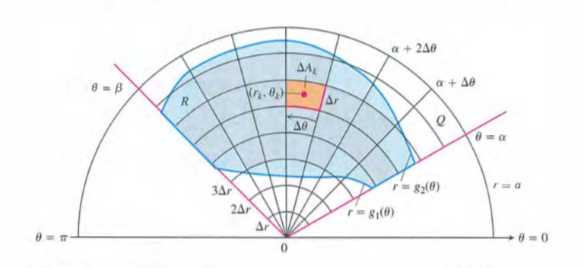
\includegraphics[scale=0.7]{m3_f12}
\end{center}

\bigskip

Copying the procedure we know well by now, we find that the integral of $f$ over $R$ is approximated by
\begin{align*}
S_n = \sum_{k=1}^n f(r_k,\theta_k)\Delta A_k.
\end{align*}
But in polar coordinates the area $\Delta A_k$ is no longer equal to $\Delta x_k \Delta y_k$. Let's look at one particular slice of the region $R$.

\bigskip

\begin{center}
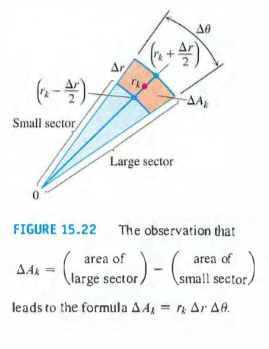
\includegraphics[scale=0.7]{m3_f13}
\end{center}

\bigskip

The area of one wedge shaped sector is the proportion of the wedge to the full circle, so its area is
\begin{align*}
A = \frac{\theta}{2\pi} \cdot \pi r^2 = \frac{1}{2} \theta r^2.
\end{align*}
Now noticing that the area of the piece $A_k$ is the area of the larger wedge minus the smaller wedge we get
\begin{align*}
A_k &= \frac{1}{2} \Delta \theta \left(r_k+\frac{\Delta r}{2}\right)^2 - \frac{1}{2} \Delta \theta \left(r_k-\frac{\Delta r}{2}\right)^2\\
&= \frac{\Delta \theta}{2} (2r_k \Delta r)\\
&= r_k \Delta r \Delta \theta.
\end{align*}

\bigskip

Thus the approximation of our integral becomes 
\begin{align*}
S_n = \sum_{k=1}^n f(r_k,\theta_k) r_k \Delta r \Delta \theta
\end{align*}
and after passing a limit as $n\to\infty$ we get
\begin{align*}
\lim_{n\to\infty} \sum_{k=1}^n f(r_k,\theta_k) r_k \Delta r \Delta \theta = \int \int_R f(r,\theta) r dr d\theta.
\end{align*}

\newpage

\hrulefill

\bigskip

\textbf{How to find bounds for double integrals in polar coordinates}
\begin{itemize}
\item[1.] Draw the region in polar coordinates.
\item[2.] Draw a line from the origin radially out to the edge of the region. Where the line enters the region is the lower bound for $r$ and where it leaves is the outer bound for $r$.
\item[3.] Determine the bounds for $\theta$ by tracing an arc through the region starting at the $x$-axis.
\end{itemize}

\bigskip

\hrulefill

\bigskip

\begin{example}
Find the limits of integration for integrating $f(r,\theta)$ over the region $R$ that lies inside the cardioid $r=1+\cos(\theta)$ and outside the circle $r=1$.

\bigskip

We start by drawing the region.

\bigskip

\begin{center}
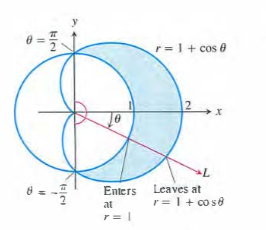
\includegraphics[scale=0.7]{m3_f14}
\end{center}

\bigskip

To find the limits of integration for $r$ we note that the line we drew through the region enters at $r=1$ and leaves at $r=1+\cos(\theta)$. To find the limits of integration for $\theta$ we must determine where the curves intersect, so we need to solve the following for $\theta$ \text{keeping in mind} the shaded region above.
\begin{align*}
1=1+\cos(\theta) &\Rightarrow 0 = \cos(\theta)\\
&\Rightarrow \theta = -\frac{\pi}{2}, \frac{\pi}{2}.
\end{align*}
Thus our integral is
\begin{align*}
\int_{-\pi/2}^{\pi/2} \int_1^{1+\cos(\theta)} f(r,\theta) rdrd\theta.
\end{align*}

\end{example}

\bigskip

\hrulefill

\bigskip

\textbf{Note:} Just like in cartesian coordinates, integrating the function $f(r,\theta) = 1$ over the region $R$ gives the area of the region.

\bigskip

\hrulefill

\bigskip

If we are given an integral that is difficult or impossible to integrate in cartesian coordinates, we should try converting the integral to polar coordinates. This is done by
\begin{align*}
\int \int_R f(x,y)dxdy = \int \int _G f(r\cos\theta),r\sin(\theta)) r dr d\theta.
\end{align*}
where $G$ is the same region as $R$ but expressed in polar coordinates.

\bigskip

\hrulefill

\bigskip

\begin{example}

Evaluate 
\begin{align*}
\int \int_R e^{x^2+y^2} dy dx
\end{align*}
where $R$ is the region bounded by the $x$-axis and the curve $y=\sqrt{1-x^2}$.

\bigskip

It may help us to sketch the region $R$.

\bigskip

\begin{center}
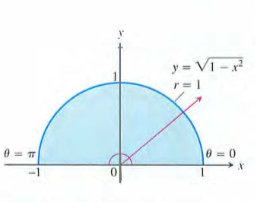
\includegraphics[scale=0.7]{m3_f15}
\end{center}

\bigskip

From this we can see the bounds on our integral are $0\leq r \leq 1$ and $0\leq \theta \leq \pi$. Now note that $x^2+y^2 = r^2$, so our integral becomes
\begin{align*}
\int \int_R e^{x^2+y^2} dydx &= \int_0^\pi \int_0^1 e^{r^2} r dr d\theta\\
&= \int_0^\pi \left[\frac{1}{2}e^{r^2}\right]_0^1 d\theta\\
&= \int_0^\pi \frac{1}{2}(e-1)d\theta\\
&= \frac{\pi}{2}(e-1).
\end{align*}

\end{example}

\bigskip

\hrulefill

\bigskip

\begin{example}

Evaluate the integral
\begin{align*}
\int_0^1 \int_0^{\sqrt{1-x^2}} (x^2+y^2)dydx.
\end{align*}
You could give this integral a shot in cartesian coordinates, but you'd quickly find it's a nightmare. Let's convert to polar coordinates. The region here is the same as the last example but only the first quadrant. That is, the region is the quarter circle with radius 1 lying in the first quadrant. Thus our integral becomes
\begin{align*}
\int_0^1 \int_0^{\sqrt{1-x^2}} (x^2+y^2)dydx &= \int_0^{\pi/2} \int_0^1 (r^2)rdrd\theta\\
&= \int_0^{\pi/2} \left[ \frac{r^4}{4}\right]_{r=0}^{r=1} d\theta\\
&= \int_0^{\pi/2} \frac{1}{4} d\theta\\
&= \frac{\pi}{8}.
\end{align*}

\end{example}

\newpage

% --------------------------------------------------------------
%                         Sec 15.5
% --------------------------------------------------------------

\section{Triple Integrals in Rectangular Coordinates (15.5)}

We'll now move to a topic that can be a little more difficult to visualize: integrating a function of three variables. Now, instead of integrating over an area in the $xy$-plane we are integrating over a volume in three dimensional space. We cannot easily discuss what this integral represents, but we can often discuss the volume over which we integrate.

\bigskip

\hrulefill

\bigskip

Consider a region $D$ in three dimensional space and say we want to integrate a function $f(x,y,z)$ over that space. Proceeding as we have in previous sections, we partition the region $D$ into small shapes, but now these shapes are $\textit{boxes}$ instead of rectangles. Each small box has volume $\Delta V_k = \Delta x_k \Delta y_k \Delta z_k$, so if we pick a point $(x_k,y_k,z_k)$ in each box then the integral is approximated by the sum
\begin{align*}
S_n = \sum_{k=1}^n F(x_k,y_k,z_k) \Delta V_k = \sum_{k=1}^n F(x_k,y_k,z_k) \Delta x_k \Delta y_k \Delta z_k.
\end{align*}
Now if we let the number of boxes go to infinity we get
\begin{align*}
\lim_{n\to\infty} S_n &= \lim_{n\to\infty} \sum_{k=1}^n F(x_k,y_k,z_k) \Delta x_k \Delta y_k \Delta z_k\\
&= \int \int \int_D F(x,y,z) dxdydz.
\end{align*}
This is called the \textbf{triple integral} of $F$ over $D$.

\bigskip

\hrulefill

\bigskip

If we integrate the function $F(x,y,z) = 1$ over a region $D$, we get the volume of the region $D$.

\bigskip

\begin{definition}
The \textbf{volume} of a closed, bounded region $D$ in space is
\begin{align*}
V= \int \int \int_D dV.
\end{align*}
\end{definition}

\bigskip

\hrulefill

\bigskip

The tricky part with these integrals is in determining the limits of integration. It doesn't matter what order we integrate with respect to (that's Fubini's Theorem) but it can sometimes be easier to integrate in a certain order. We'll outline one of the most common orders to start with.

\bigskip

\textbf{Integrating in the Order $dzdydx$}
\begin{itemize}
\item[1.] If you can, sketch the region $D$ along with its ``shadow" $R$. This step is not always necessary but can be helpful
\item[2.] To find the bounds for $z$, imagine drawing a vertical line (parallel to $z$ axis) through the region. Where this line enters the region is the lower bound, and where it exits is the upper bound. These bounds will likely be functions of $x$ and $y$ (i.e. $z=f_1(x,y)$ and $z=f_2(x,y)$).
\item[3.] To find the bounds for $y$, draw a line through $R$ parallel to the $y$ axis. Where this line enters $R$ is the lower bound, and where it exits is the upper bound. These bounds will likely be a function of $x$ (i.e. $y=g_1(x)$ and $y=g_2(x)$).
\item[4.] Choose $x$ limits that include all lines through $R$ parallel to the $y$-axis. These will be numbers (i.e. $x=a$ and $x=b$).
\end{itemize}

\bigskip

If we choose to integrate in this order, we will get something like
\begin{align*}
\int_{x=a}^{x=b} \int_{y=g_1(x)}^{y=g_2(x)} \int_{z=f_1(x,y)}^{z=f_2(x,y)} F(x,y,z) dzdydx.
\end{align*}

\bigskip

\hrulefill

\bigskip

\begin{definition}
The \textbf{average value} of $F$ over $D$ is
\begin{align*}
A_f = \frac{1}{\text{volume of} \ D} \int \int \int_D F dV.
\end{align*}
\end{definition}

\bigskip

\hrulefill

\bigskip

\begin{example}
Find the average value of $F(x,y,z) = xyz$ throughout the cubical region $D$ bounded by the coordinate planes and the planes $x=2, y=2$ and $z=2$ in the first octant.

\bigskip

We first need to find the volume of the region $D$, so note that our region is the following cube. (Draw picture of cube). We don't need to set up an integral to find this volume, we know it is $V=8$. Thus our average value is
\begin{align*}
V_f &= \frac{1}{8} \int_0^2 \int_0^2 \int_0^2 xyzdzdydx\\
&= \frac{1}{8} \int_0^2 \int_0^2 \left[ xy\frac{z^2}{2} \right]_{z=0}^{z=2} dy dx\\
&= \frac{1}{8} \int_0^2 \int_0^2 2xy dy dx\\
&= \frac{1}{8} \int_0^2 \left[2x\frac{y^2}{2}\right]_{y=0}^{y=2} dx\\
&= \frac{1}{8} \int_0^2 4x dx\\
&= \frac{1}{8} \left[2x^2\right]_0^2\\
&= 1.
\end{align*}
\end{example}

\bigskip

\hrulefill

\bigskip

\begin{example}
Set up, but do not evaluate, the integral that gives the volume of the region $D$ enclosed by the surfaces $z=x^2+3y^2$ and $z=8-x^2-y^2$.

\bigskip

It would be difficult to sketch the region $D$ here, so we will just sketch the region $R$. To determine what $R$ is, we need to know where the surfaces intersect. Note that
\begin{align*}
x^2+3y^2 &= 8-x^2-y^2\\
\Rightarrow x^2+2y^2&=4\\
\Rightarrow \frac{x^2}{4}+\frac{y^2}{2} &=1.
\end{align*}

\bigskip

\begin{center}
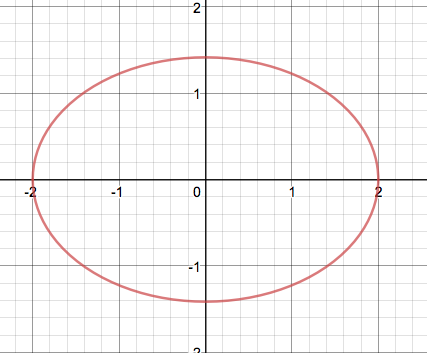
\includegraphics[scale=0.7]{m3_f16}
\end{center}

\bigskip

To find the bounds for the variable $z$ imagine drawing a line through the origin (which we know is in $R$) that is parallel to the $z$ axis. We can see that this line passes through $z=x^2+3y^2$ first then through $z=8-x^2-y^2$. To find the bounds for the $y$-axis note that a line through $R$ parallel to the $y$ axis first passes through $y=-\sqrt{(4-x^2)/2}$ then through $y=\sqrt{(4-x^2)/2}$. The bounds for $x$ we can see from our drawing are $x=-2$ and $x=2$. Therefore we get
\begin{align*}
V &= \int \int \int_D dzdydz\\
&= \int_{-2}^2 \int_{-\sqrt{(4-x^2)/2}}^{\sqrt{(4-x^2)/2}} \int_{x^2+3y^2}^{8-x^2-y^2} dzdydz.
\end{align*}

\end{example}

% Include another example or two that shows how to switch the order when one direction is tough. Ask
% John or Joshua if they have any good examples for this.

\newpage

% --------------------------------------------------------------
%                         Sec 15.6
% --------------------------------------------------------------

\section{Moments and Centers of Mass (15.6)}

If $\delta(x,y,z)$ is the density (mass per unit volume) of an object occupying a region $D$ in space, then we could think of splitting the object into a number $n$ of small cubes. The mass of each cube is then $\Delta m_k = \delta(x_k,y_k,z_k) \Delta V_k$. Finding the full mass of the object gives
\begin{align*}
M = \sum_{k=1}^n \Delta m_k = \lim_{n\to\infty} \sum_{k=1}^n \delta (x_k,y_k,z_k) \Delta V_k = \int \int \int_D \delta(x,y,z)dV.
\end{align*}

\bigskip

\hrulefill

\bigskip

This formula for mass is sometimes called the \textbf{zeroeth moment} of the density function $\delta$, in contrast to the \textbf{first moment}. The first moment about the ${yz}-plane$ is the integral
\begin{align*}
M_{yz} = \int \int \int_D x\delta(x,y,z)dV.
\end{align*}
First moments allow us to find the \textbf{center of mass} of an object. For example, the $x$-coordinate of the center of mass of an object is
\begin{align*}
\overline{x} = M_{yz}/M.
\end{align*}

\bigskip

\hrulefill

\bigskip

\textbf{Three-Dimensional Solid}
\begin{align*}
\textbf{Mass: } M&=\int\int\int_D \delta(x,y,z) dV\\
\textbf{First moments: } M_{yz} &= \int \int \int_D x\delta(x,y,z)dV\\ M_{xz} &= \int \int \int_D y\delta(x,y,z)dV\\ M_{xy} &= \int \int \int_D z\delta(x,y,z)dV\\
\textbf{Center of mass: } \overline{x} &= \frac{M_{yz}}{M}, \ \ \overline{y} = \frac{M_{xz}}{M}, \ \ \overline{z} - \frac{M_{xy}}{M}
\end{align*}

\bigskip

\textbf{Two-Dimensional Plate}
\begin{align*}
\textbf{Mass: } M&=\int\int_R \delta(x,y) dA\\
\textbf{First moments: } M_{y} &= \int \int_R x\delta(x,y)dA\\ M_{x} &= \int \int_R y\delta(x,y)dA\\ 
\textbf{Center of mass: } \overline{x} &= \frac{M_{y}}{M}, \ \ \overline{y} = \frac{M_{x}}{M}
\end{align*}

\bigskip

\hrulefill

\bigskip

\begin{example}
A thin plate covers the triangular region bounded by the $x$-axis and the lines $x=1$ and $y=2x$ in the first quadrant. The plate's density at the point $(x,y)$ is $\delta(x,y) = 6x+6y+6$. Find the mass and the center of mass of the plate.

\bigskip

First we make a sketch of the region.

\bigskip

\begin{center}
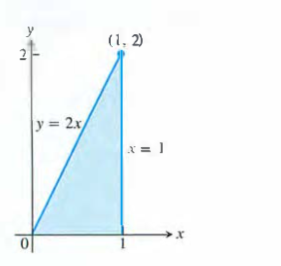
\includegraphics[scale=0.7]{m3_f17}
\end{center}

\bigskip

Now for the mass we have
\begin{align*}
M &= \int \int_R \delta(x,y)dA\\
&= \int_0^1 \int_0^{2x} (6x+6y+6)dydx\\
&= \int_0^1 \left[6xy+3y^2+6y\right]_{y=0}^{y=2x} dx\\
&= \int_0^1(12x^2+12x^2+12x)dx\\
&= \int_0^1(24x^2+12x)dx\\
&= \left[8x^3+6x^2\right]_0^1\\
&= 14.
\end{align*}
For the center of mass calculations we get
\begin{align*}
\overline{x} &= \frac{M_y}{M}\\
&= \frac{1}{14} \int \int_R x\delta(x,y)dA\\
&= \frac{1}{14} \int_0^1 \int_0^{2x} (6x^2+6xy+6x)dydx\\
&= \frac{1}{14} \int_0^1 \left[6x^2y+3xy^2+6xy\right]_{y=0}^{y=2x} dx\\
&= \frac{1}{14} \int_0^1(12x^3+12x^3+12x^2)dx\\
&= \frac{1}{14} \int_0^1(24x^3+12x^2)dx\\
&= \frac{1}{14} \left[6x^4+4x^3\right]_0^1\\
&= \frac{10}{14}=\frac{5}{7}.
\end{align*}
and
\begin{align*}
\overline{y} &= \frac{M_x}{M}\\
&= \frac{1}{14} \int \int_R y\delta(x,y)dA\\
&= \frac{1}{14} \int_0^1 \int_0^{2x} (6xy+6y^2+6y)dydx\\
&= \frac{1}{14} \int_0^1 \left[3xy^2+2y^3+3y^2\right]_{y=0}^{y=2x} dx\\
&= \frac{1}{14} \int_0^1(12x^3+16x^3+12x^2)dx\\
&= \frac{1}{14} \int_0^1(28x^3+12x^2)dx\\
&= \frac{1}{14} \left[7x^4+4x^3\right]_0^1\\
&= \frac{11}{14}.
\end{align*}
Thus the center of mass is $(\overline{x},\overline{y}) = \left(\frac{5}{7},\frac{11}{14}\right)$.

\end{example}

\bigskip

\hrulefill

\bigskip

% Include another example that involves using symmetry to deduce coordinates of center of mass without computing any integrals.

\newpage

% --------------------------------------------------------------
%                         Sec 15.7
% --------------------------------------------------------------

\section{Triple Integrals in Cylindrical and Spherical Coordinates (15.7)}

Cartesian coordinates in three dimensions are great for dealing with rectangular-prism type shapes. But if we instead want to work with something like a cylinder, cone or sphere then Cartesian coordinates become quite difficult to work with. Just like in two dimensions we could ``redraw" our grid lines using polar coordinates, we will now look at ``redrawing" our grid lines in three dimensions using other coordinate systems.

\bigskip

\hrulefill

\bigskip

\begin{definition}
\textbf{Cylindrical coordinates} represent a point $P$ in space by ordered triples $(r,\theta,z)$ in which
\begin{itemize}
\item[1.] $r$ and $\theta$ are polar coordinates for the vertical projection of $P$ on the $xy$-plane
\item[2.] $z$ is the rectangular vertical coordinate.
\end{itemize}
\end{definition}

\bigskip

\begin{center}
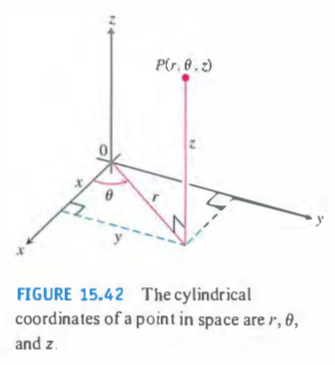
\includegraphics[scale=0.7]{m3_f18}
\end{center}

\bigskip

\hrulefill

\bigskip

\begin{definition}{Equations Relating Rectangular and Cylindrical Coordinates}
\begin{align*}
x=&r\cos(\theta), \ \ y=r\sin(\theta), \ \ z=z,\\
&r^2=x^2+y^2, \ \ \tan(\theta) = y/x
\end{align*}
\end{definition}

\bigskip

\hrulefill

\bigskip

\begin{example}
Plot the equations $r=4$, $\theta = \pi/3$, and $z=2$ in cylindrical coordinates.

\bigskip

(Plot each graph). $r=4$ is a cylinder with radius $4$ since we take a circle in 2-dimensions and project it up and down! $\theta=\pi/3$ is a plane containing the $z$-axis along the line $\theta=\pi/3$. $z=2$ is a plane perpendicular to the $z$-axis.
\end{example}

\bigskip

\hrulefill

\bigskip

Suppose we want to integrate a function defined over a region $D$ in cylindrical coordinates. Now when we partition our space it is into small wedges instead of cubes! The integral then is approximated by
\begin{align*}
S_n = \sum_{k=1}^n f(r_k,\theta_k, z_k) \Delta V_k.
\end{align*}
What is $\Delta V_k$?

\bigskip

\begin{center}
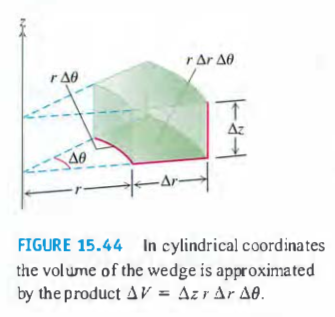
\includegraphics[scale=0.7]{m3_f19}
\end{center}

\bigskip

We saw in the polar coordinates section that the area in 2-d for one of these wedges is $\Delta A_k = r_k \Delta r_k \Delta \theta_k$. So the volume of the 3-d wedge is $\Delta V_k = \Delta z_k r_k \Delta r_k \Delta \theta_k$. Thus we have
\begin{align*}
S_n = \sum_{k=1}^n f(r_k,\theta_k, z_k) \Delta z_k r_k \Delta r_k \Delta \theta_k
\end{align*}
giving
\begin{align*}
\lim_{n\to\infty} S_n = \int\int\int_D f(r,\theta,z) dV = \int\int\int f(r,\theta,z) rdrd\theta dz
\end{align*}

\bigskip

\hrulefill

\bigskip

\textbf{Steps for Integrating in cylindrical coordinates}
\begin{itemize}
\item[1.] If you can, draw the region $D$.
\item[2.] Find the $z$ limits of integration by drawing a line parallel to the $z$-axis through your region. Where the line enters the region ($z=g_1(r,\theta)$) is your lower bound, where it exits ($z=g_2(r,\theta)$) is the upper bound.
\item[3.] Find the $r$ limits of integration by drawing a ray through the projection of $D$ onto two-dimensions $R$. Where the ray enters the region is the lower bound $r=h_1(\theta)$ and where it exits is the upper bound $r=h_2(\theta)$.
\item[4.] Find the $\theta$ limits of integration by sweeping your ray across $R$. You should get some bounds that look like $\theta=\alpha$ and $\theta=\beta$. Your final integral will look like
\begin{align*}
\int\int\int_D f(r,\theta,z) dV = \int_{\theta=\alpha}^{\theta=\beta} \int_{r=h_1(\theta)}^{r=h_2(\theta)} \int_{g_1(r,\theta)}^{g_2(r,\theta)} f(r,\theta,z) dz r dr d\theta.
\end{align*}
\end{itemize}

\bigskip

\hrulefill

\bigskip

\begin{example}
Find the limits of integration in cylindrical coordinates for integrating a function $f(r,\theta,z)$ over the region $D$ bounded below by the plane $z=0$, laterally by the circular cylinder $x^2+(y-1)^2 = 1$, and above by the paraboloid $z=x^2+y^2$.

\bigskip

The region in question here looks like the following.

\bigskip

\begin{center}
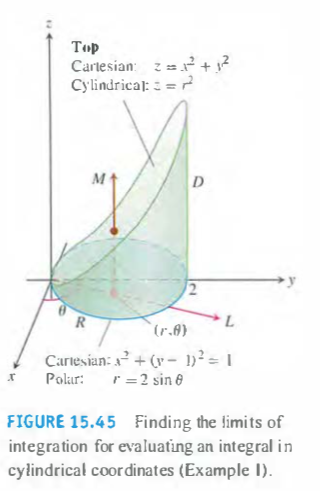
\includegraphics[scale=0.7]{m3_f20}
\end{center}

\bigskip

It will be helpful here to determine the region of projection $R$ on the $xy$-plane. The region is given in cartesian coordinates by $x^2+(y-1)^2=1$. Converting this to polar coordinates gives
\begin{align*}
x^2+(y-1)^2&=1\\
\Rightarrow x^2+y^2-2y+1&=1\\
\Rightarrow r^2-2r\sin(\theta)&=0\\
\Rightarrow r&=2\sin(\theta).
\end{align*}
Now following our steps from above, we see that a vertical line through the region first crosses $z=0$ then crosses $z=x^2+y^2=r^2$. A ray from the origin passes through $R$ at $r=0$ and then again at $r=2\sin(\theta)$. Our bounds for $\theta$ here are from $\theta=0$ to $\theta=\pi$. Thus our integral is
\begin{align*}
\int \int \int_D f(r,\theta,z)dV = \int_0^\pi \int_0^{2\sin(\theta)} \int_0^{r^2} f(r,\theta,z) dz r dr d\theta.
\end{align*}
\end{example}

\bigskip

\hrulefill

\bigskip

This isn't the only coordinate system we can use in three-dimensional space.

\bigskip

\begin{definition}
\textbf{Spherical coordinates} represent a point $P$ in space by ordered triples $(\rho, \phi,\theta)$ in which
\begin{itemize}
\item[1.] $\rho$ is the distance from $P$ to the origin ($\rho>0$)
\item[2.] $\phi$ is the angle $\vec{OP}$ makes with the positive $z$-axis ($0\leq \phi \leq \pi$)
\item[3.] $\theta$ is the angle from cylindrical coordinates ($0\leq \theta \leq 2\pi$).
\end{itemize}
\end{definition}

\bigskip

\begin{center}
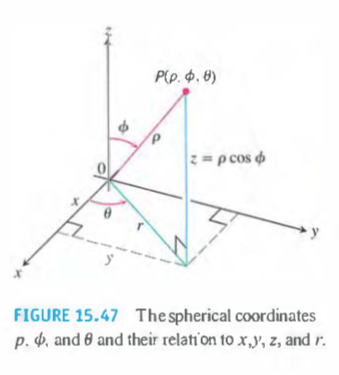
\includegraphics[scale=0.7]{m3_f21}
\end{center}

\bigskip

\hrulefill

\bigskip

\begin{definition}{Equations Relating Spherical Coordinates to Cartesian and Cylindrical Coordinates}
\begin{align*}
r&=\rho\sin(\phi), \ \ x=r\cos(\theta), \ \ \rho\sin(\phi)\cos(\theta),\\
z&=\rho\cos(\phi), \ \ y=r\sin(\theta), \ \ \rho\sin(\phi)\sin(\theta),\\
\rho &= \sqrt{x^2+y^2+z^2} = \sqrt{r^2+z^2}.
\end{align*}
\end{definition}

\bigskip

\hrulefill

\bigskip

\begin{example}
Plot the equations $\rho=2$, $\phi = \pi/2$, and $\theta=\pi/4$ in cylindrical coordinates.

\bigskip

(Plot each graph). $\rho=2$ is a sphere with radius $2$. $\phi=\pi/2$ is a cone whose vertex lies at the origin and whose axis lies along the $z$-axis. $\theta = \pi/4$ is the half-plane containing the $z$-axis and making an angle of $\pi/4$ with the positive $x$-axis.
\end{example}

\bigskip

\hrulefill

\bigskip

Suppose we want to integrate a function defined over a region $D$ in spherical coordinates. Now when we partition our space it is into small spherical wedges instead of cubes! The integral then is approximated by
\begin{align*}
S_n = \sum_{k=1}^n f(\rho_k, \phi_k, \theta_k) \Delta V_k.
\end{align*}
Finding $\Delta V_k$ in this case is trickier than for cylindrical coordinates. It turns out this volume is $\Delta V_k = \rho_k^2\sin(\phi_k)\Delta \rho_k \Delta \phi_k \Delta \theta_k$. Thus we have
\begin{align*}
S_n = \sum_{k=1}^n f(\rho_k, \phi_k, \theta_k) \rho_k^2\sin(\phi_k) \Delta \rho_k \Delta \phi_k \Delta \theta_k
\end{align*}
giving
\begin{align*}
\lim_{n\to\infty} S_n = \int\int\int_D f(\rho,\phi,\theta)dV = \int\int\int_D f(\rho,\phi,\theta) \rho^2 \sin(\phi)d\rho d\phi d\theta.
\end{align*}

\bigskip

\hrulefill

\bigskip

\textbf{Steps for Integrating in spherical coordinates}
\begin{itemize}
\item[1.] If you can, draw the region $D$.
\item[2.] Find the $\rho$ limits of integration by drawing a ray from the origin through the region. Where the ray enters the region ($\rho=g_1(\phi,\theta)$) is your lower bound, where it exits ($\rho=g_2(\phi,\theta)$) is the upper bound.
\item[3.] Find the $\phi$ limits of integration by either tracing out $\phi$ to the edge of the region to get $\phi=0$ to $\phi=\phi_{\text{max}}$ or if your region has a hole trace out $\phi$ through the region to get $\phi=\phi_{\text{min}}$ and $\phi=\phi_{\text{max}}$.
\item[4.] Find the $\theta$ limits of integration by sweeping your ray across $R$. You should get some bounds that look like $\theta=\alpha$ and $\theta=\beta$. Your final integral will look like
\begin{align*}
\int\int\int_D f(r,\theta,z) dV = \int_{\theta=\alpha}^{\theta=\beta} \int_{\phi=\phi_{\text{min}}}^{\phi_{\text{max}}} \int_{\rho=g_1(\phi,\theta)}^{\rho=g_2(\phi,\theta)} f(\rho,\phi,\theta) \rho^2\sin(\phi)d\rho d\phi d\theta.
\end{align*}
\end{itemize}

\bigskip

\hrulefill

\bigskip

\begin{example}
Find the volume of the ``ice cream cone" $D$ cut from the solid sphere $\rho \leq 1$ by the cone $\phi = \pi/3$.

\bigskip

A sketch of the region is given below.

\bigskip

\begin{center}
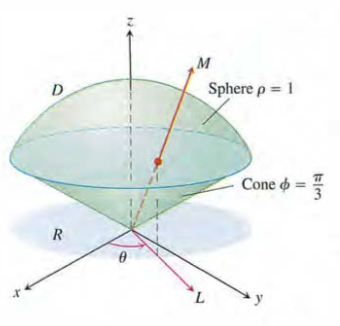
\includegraphics[scale=0.7]{m3_f22}
\end{center}

\bigskip

From our drawing we see that the $\rho$ limits of integration are $\rho=0$ and $\rho=1$. We can also see that the region for $\phi$ is $\phi=0$ to $\phi=\pi/3$. Finally we also identify that $\theta$ runs from $\theta=0$ to $\theta=2\pi$. Thus our volume is
\begin{align*}
V &= \int\int\int_D \rho^2\sin(\phi)d\rho d\phi d\theta\\
&= \int_0^{2\pi} \int_0^{\pi/3} \int_0^1 \rho^2\sin(\phi)d\rho d\phi d\theta\\
&= \int_0^{2\pi} \int_0^{\pi/3} \left[\frac{\rho^3}{3}\right]_0^1 d\phi d\theta\\
&= \int_0^{2\pi} \int_0^{\pi/3} \frac{1}{3} \sin(\phi)d\phi d\theta\\
&= \int_0^{2\pi} \left[-\frac{1}{3}\cos(\phi)\right]_0^{\pi/3} d\theta\\
&= \int_0^{2\pi} \left(-\frac{1}{6} + \frac{1}{3} \right)d\theta\\
&= \frac{\pi}{3}.
\end{align*}

\end{example}

\bigskip

\hrulefill

\bigskip

% Include two more examples of switching from cartesian to cylindrical or spherical.

\newpage

% --------------------------------------------------------------
%                         Sec 15.8
% --------------------------------------------------------------

\section{Substitutions in Multiple Integrals (15.8)}

Recall from Calc I that some integrals were much easier to solve after performing a $u$-substitution. We have an equivalent idea for integrals of functions in 2-dimensions, but the process is a little bit different.

\bigskip

Say we start with a region $R$ in cartesian coordinates and we would like to find the integral of $f$ over $R$. That is, we want to find
\begin{align*}
\int\int_R f(x,y)dxdy.
\end{align*}
There are times this might be hard to do, so lets instead say we substitute for $x$ and $y$ using the relationships $x=g(u,v)$ and $y=h(u,v)$. Our region $R$ is no longer necessarily the same!

\bigskip

\begin{center}
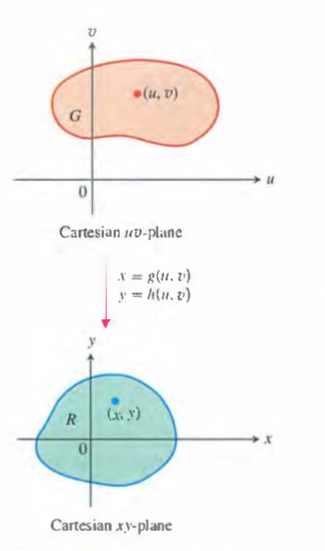
\includegraphics[scale=0.7]{m3_f23}
\end{center}

\bigskip

It turns out we have
\begin{align*}
\int\int_R f(x,y)dxdy = \int\int_G f(g(u,v),h(u,v))|J(u,v)|dudv
\end{align*}
where $J(u,v)$ is the \textbf{Jacobian} of the coordinate transformation.

\bigskip

\hrulefill

\bigskip

\begin{definition}
The \textbf{Jacobian} or \textbf{Jacobian determinant} of the coordinate transformation $x=g(u,v)$, $y=h(u,v)$ is
\begin{align*}
J(u,v) = \begin{vmatrix} \frac{\partial x}{\partial u} & \frac{\partial x}{\partial v} \\ \frac{\partial y}{\partial u} & \frac{\partial y}{\partial v} \end{vmatrix} = \frac{\partial x}{\partial u}\frac{\partial y}{\partial v}-\frac{\partial x}{\partial v}\frac{\partial y}{\partial u}.
\end{align*}
\end{definition}

\bigskip

\hrulefill

\bigskip

We've actually already seen a coordinate change/substitution in this class, as the next example shows.

\begin{example}
Find the Jacobian for the polar coordinate transformation $x=r\cos(\theta)$, $y=r\sin(\theta)$ and then write the Cartesian integral $\int\int\int_R f(x,y)dxdy$ as a polar integral.

\bigskip

This drawing shows how the coordinate system is transformed.

\bigskip

\begin{center}
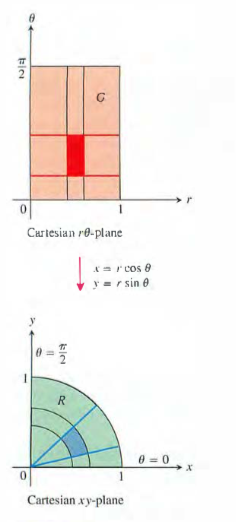
\includegraphics[scale=0.7]{m3_f24}
\end{center}

\bigskip

For the Jacobian calculation we have
\begin{align*}
J(r,\theta) &= \begin{vmatrix} \cos(\theta) & -r\sin(\theta) \\ \sin(\theta) & r\cos(\theta) \end{vmatrix}\\
&=r(\cos^2(\theta)+\sin^2(\theta))\\
&=r.
\end{align*}
Therefore our integral is
\begin{align*}
\int\int_R f(x,y)dxdy = \int\int_G f(r\cos(\theta),r\sin(\theta)) r dr d\theta.
\end{align*}

\end{example}

\bigskip

\hrulefill

\bigskip

\textbf{Steps for substitutions in multiple integrals:}
\begin{itemize}
\item[1.] If you can, draw the region before and after the transformation. Find the new bounds of integration.
\item[2.] Compute the Jacobian.
\item[3.] Apply the substitution to the integrand.
\end{itemize}

\bigskip

\hrulefill

\bigskip

\begin{example}
Evaluate
\begin{align*}
\int_0^4 \int_{y/2}^{(y/2)+1} \frac{2x-y}{2}dxdy
\end{align*}
by applying the transformation
\begin{align*}
u=\frac{2x-y}{2}, \ \ v=\frac{y}{2}.
\end{align*}
In this case we can draw the region before and after the transformation. To do this, we need to consider what our bounds for the integral over $u$ and $v$ will be. First note that
\begin{align*}
u=\frac{2x-y}{2} &\Rightarrow 2u=2x-y\\
&\Rightarrow 2u=2x-2v\\
&\Rightarrow u+v=x \ \ \text{and} \ \ y=2v.
\end{align*}
Using these we find that
\begin{align*}
x=y/2 \Rightarrow u+v=2v/2=v \Rightarrow &u=0\\
x=(y/2)+1 \Rightarrow u+v=(2v/2)+1=v+1 \Rightarrow &u=1\\
y=0 \Rightarrow 2v=0 \Rightarrow &v=0\\
y=4 \Rightarrow 2v=4 \Rightarrow &v=2.
\end{align*}
Thus after being transformed our region is now a rectangle in $u$-$v$ space! 

\bigskip

\begin{center}
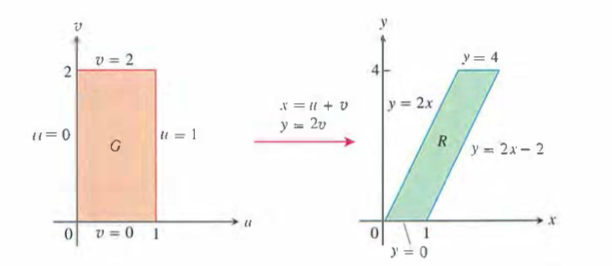
\includegraphics[scale=0.7]{m3_f25}
\end{center}

\bigskip

Now to find the Jacobian we have
\begin{align*}
J(u,v) &= \begin{vmatrix} \frac{\partial}{\partial u} (u+v) & \frac{\partial}{\partial v} (u+v)\\ \frac{\partial}{\partial u} (2v) & \frac{\partial}{\partial v} (2v) \end{vmatrix}\\
&= \begin{vmatrix} 1 & 1 \\ 0 & 2 \end{vmatrix} = 2.
\end{align*}
Therefore we have
\begin{align*}
\int_0^4 \int_{y/2}^{(y/2)+1} \frac{2x-y}{2}dxdy &= \int_{v=0}^{v=2} \int_{u=0}^{u=1} u |J(u,v)|dudv\\
&= \int_0^2 \int_0^1 2u du dv\\
&= \int_0^2 \left[u^2\right]_0^1 dv\\
&=\int_0^2 dv\\
&=2.
\end{align*}

\end{example}

\bigskip

\hrulefill

\bigskip

\begin{example}
Evaluate the integral
\begin{align*}
\int_1^2 \int_{1/y}^y \sqrt{\frac{y}{x}} e^{\sqrt{xy}} dxdy.
\end{align*}

\bigskip

We should make the substitutions here $u=\sqrt{xy}, v= \sqrt{y/x}$. Squaring these equations gives $u^2=xy$ and $v^2=y/x$. Now see that
\begin{align*}
u^2=xy &\Rightarrow \frac{yu^2}{x} = y^2\\
&\Rightarrow u^2v^2=y^2\\
&\text{and}\\
u^2=xy &\Rightarrow \frac{xu^2}{y} = x^2\\
&\Rightarrow \frac{u^2}{v^2} = x^2.
\end{align*}
This means
\begin{align*}
x=\frac{u}{v} \ \ \text{and} \ \ y=uv.
\end{align*}
Our region here is not a rectangle, as shown in this drawing.

\bigskip

\begin{center}
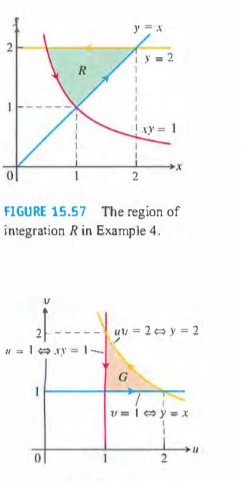
\includegraphics[scale=0.7]{m3_f26}
\end{center}

\bigskip

So see that the left bound $xy=1$ becomes $u=\sqrt{xy}=\sqrt{1}=1$ and $v=\sqrt{y^2} = y$ and since $1\leq y \leq 2$ we know that $1\leq v \leq 2$. The right bound $y=x$ becomes $v=\sqrt{y/y} = 1$ and $u=y$ and again since $1\leq y \leq 2$ we know that $1\leq u \leq 2$. Lastly the top bound $y=2$ implies that $uv = \sqrt{2x}\sqrt{2/x} = 2$ again with $1\leq u \leq 2$. Thus before calculating the Jacobian we have
\begin{align*}
\int_1^2 \int_{1/y}^y \sqrt{\frac{y}{x}} e^{\sqrt{xy}} dxdy = \int_1^2 \int_1^{2/u} ve^u |J(u,v)| dv du.
\end{align*}
Now calculating the Jacobian gives
\begin{align*}
J(u,v) &= \begin{vmatrix} \frac{1}{v} & -\frac{u}{v^2} \\ v & u \end{vmatrix}\\
&= \frac{u}{v} + \frac{u}{v} = \frac{2u}{v}.
\end{align*}
Therefore our integral is
\begin{align*}
\int_1^2 \int_{1/y}^y \sqrt{\frac{y}{x}} e^{\sqrt{xy}} dxdy &= \int_1^2 \int_1^{2/u} 2ue^u dv du\\
&= 2 \int_1^2 \left[vue^u\right]_{v=1}^{v=2/u} du\\
&= 2 \int_1^2 (2e^u-ue^u)du\\
&= 2\int_1^2 (2-u)e^udu\\
&=2\left(\left[(2-u)e^u\right]_1^2 + \int_1^2 e^u du\right)\\
&= -2e+2e^2-2e\\
&= 2e^2-4e.
\end{align*}

\end{example}

\bigskip

\hrulefill

\bigskip

%Add another example with an elliptic transformation

Note that we could also do these transformations for integrals over three variables. In fact we already have with cylindrical and spherical coordinates!

\newpage

% --------------------------------------------------------------
%                         Sec 16.1
% --------------------------------------------------------------

\section{Line Integrals (16.1)}

Line integrals deal with the concept of integrating a multi-dimensional function over an arbitrary curve in its domain. This intuition implies that line integrals are one dimensional, they just aren't over an interval $[a,b]$ like we're used to seeing.

\bigskip

Suppose we want to integrate a real-valued function$f$ over the curve $C$ lying in the domain of $f$ and parametrized by $\bm{r}(t) = g(t) \bm{i} + h(t) \bm{j} + k(t) \bm{k}$, $a\leq t\leq b$. We break the curve up into small segments like the following.

\bigskip

\begin{center}
\includegraphics[scale=0.7]{m3_f27}
\end{center}

\bigskip

Now the value of the integral is approximated by the value of $f$ at some point in the interval multiplied by the length of the interval.
\begin{align*}
S_n = \sum_{k=1}^n f(x_k,y_k,z_k)\Delta s_k.
\end{align*}
When the limit of $S_n$ exists as $n\to\infty$ we get the following definition.

\bigskip

\begin{definition}
If $f$ is defined on a curve $C$ given parametrically by $\bm{r}(t) = g(t)\bm{i}+h(t)\bm{j}+k(t)\bm{k}$, $a\leq t \leq b$, then the \textbf{line integral of} $f$ \textbf{over} $C$ is
\begin{align*}
\int_C f(x,y,z)ds = \lim_{n\to\infty} \sum_{k=1}^n f(x_k,y_k,z_k) \Delta s_k,
\end{align*}
provided the limit exists.
\end{definition}

\bigskip

\hrulefill

\bigskip

If the function $f$ is continuous on the smooth curve $C$, we can actually write the line integral in a nice way. Remember that the arc length of a curve in space is
\begin{align*}
s(t) = \int_a^t |\bm{v}(\tau)|d\tau.
\end{align*}
So $ds = |\bm{v}(t)|dt$ by the Fundamental Theorem of Calculus. Thus we have
\begin{align*}
\int_C f(x,y,z)ds = \int_a^b f(g(t),h(t),k(t)) |\bm{v}(t)|dt.
\end{align*}

\bigskip

\hrulefill

\bigskip

\textbf{How to Evaluate a Line Integral}
To integrate a continuous function $f(x,y,z)$ over a curve $C$:
\begin{itemize}
\item[1.] Find a smooth parametrization of $C$,
\begin{align*}
\bm{r}(t) = g(t)\bm{i}+h(t)\bm{j}+k(t)\bm{k}, \ \ a\leq t \leq b
\end{align*}
\item[2.] Evaluate the integral as
\begin{align*}
\int_C f(x,y,z)ds = \int_a^b f(g(t),h(t),k(t))|\bm{v}(t)|dt.
\end{align*}
\end{itemize}

\bigskip

\hrulefill

\bigskip

The following animation may help with the intuition here.
http: //tinyurl.com/k63c6fg.

\bigskip

\hrulefill

\bigskip

A question: what happens if we integrate the function $f(x,y,z) = 1$ over a curve? Answer: we get the arc length!

\bigskip

\hrulefill

\bigskip

\begin{example}
Find the line integral of the function $f(x,y) = 2x+3y^2$ over the line segment $y=x, \ 0\leq x \leq 4$.

\smallskip

We first need to find a parametrization. In cases where we have a straight line segment connecting two points $P$ and $Q$ one possible parametrization is
\begin{align*}
\bm{r}(t) = \bm{P}(1-t)+\bm{Q}t, \ \ 0\leq t \leq 1
\end{align*}
So here we would have
\begin{align*}
\bm{r}(t) &= \langle 0,0 \rangle(1-t) + \langle 4,4 \rangle t\\
&= \langle 4t, 4t \rangle
\end{align*}
where $0\leq t \leq 1$. So our line integral is
\begin{align*}
\int_C f(x,y) ds &= \int_0^1 f(4t,4t) |\langle 4t, 4t \rangle| dt\\
&= \int_0^1 (8t+48t^2)\left(\sqrt{(4)^2+(4)^2}\right)dt\\
&= \int_0^1 (8t+48t^2)(\sqrt{32})dt\\
&= \int_0^1 (8\sqrt{32}t+48\sqrt{32}t^2)dt\\
&= \left[\frac{8}{2}\sqrt{32}t^2+16\sqrt{32}t^3\right]_0^1\\
&=4\sqrt{32}+16\sqrt{32}\\
&=80\sqrt{2}.
\end{align*}
\end{example}

\bigskip

\hrulefill

\bigskip

\begin{example}
Set up (but do not evaluate) the line integral of the function $f(x,y) = 2x+3y^2$ over the curve $y=x^2, \ 0\leq x \leq 2$.

\smallskip

We first need to find a parametrization. Here our curve is not a straight line. In these cases it is usually easiest to start with $\bm{r}(t) = \langle x(t),y(t)\rangle$ and then use substitution. When $y$ is given as a function of $x$, we can always let $x=t$ and then let $y=f(t)$. So in this case we would have
\begin{align*}
\bm{r}(t) &= \langle t, t^2 \rangle
\end{align*}
where $0\leq t \leq 2$. So our line integral is
\begin{align*}
\int_C f(x,y) ds&= \int_0^1 f(t,t^2) |\langle t, t^2 \rangle| dt\\
&= \int_0^1 (2t+3t^2)\sqrt{t^2+t^4} dt.
\end{align*}
\end{example}

\bigskip

\hrulefill

\bigskip

\begin{example}
Integrate $f(x,y,z) = x-3y^2+z$ over the line segment $C$ joining the origin to the point $(1,1,1)$.

\bigskip

Our straight line parametrization gives
\begin{align*}
\bm{r}(t) &= \langle 0,0,0 \rangle (1-t) + \langle 1,1,1 \rangle t\\
&= \langle t,t,t \rangle, \ \ 0\leq t \leq 1.
\end{align*}
Thus our line integral is
\begin{align*}
\int_C f(x,y,z)ds &= \int_0^1 f(t,t,t) |\langle t,t,t \rangle| dt\\
&= \int_0^1 (t-3t^2+t) \sqrt{3}dt\\
&= \sqrt{3} \int_0^1 (2t-3t^2) dt\\
&= \sqrt{3} \left[ t^2-t^3 \right]_0^1\\
&=0.
\end{align*}
\end{example}

\bigskip

\hrulefill

\bigskip

If our curve $C$ consists of a finite number of smooth curve $C_1, C_2, ..., C_n$ attached end to end then the integral of $f$ over $C$ is the sum of the integrals over each curve:
\begin{align*}
\int_C fds = \int_{C_1} fds + \int_{C_2} fds + ... + \int_{C_s} fds.
\end{align*}

\bigskip

\hrulefill

\bigskip

\begin{example}
Consider again the previous example, but now integrate over the region $C=C_1 \cup C_2$ given in the following drawing.

\bigskip

\begin{center}
\includegraphics[scale=0.7]{m3_f28}
\end{center}

\bigskip

We can parametrize $C_1$ and $C_2$ using our straight line parametrization.
\begin{align*}
C_1: \bm{r}(t) &= \langle 0,0,0 \rangle (1-t) + \langle 1,1,0 \rangle t\\
&= \langle t,t,0 \rangle\\
C_2: \bm{r}(t) &= \langle 1,1,0 \rangle (1-t) + \langle 1,1,1 \rangle t\\
&= \langle 1-t, 1-t, 0 \rangle + \langle t,t,t \rangle\\
&= \langle 1,1, t \rangle
\end{align*}
where $0\leq t\leq 1$ for both curve. Thus our integral is
\begin{align*}
\int_C f(x,y,z)ds &= \int_{C_1} f(x,y,z)ds + \int_{C_2} f(x,y,z)ds\\
&= \int_0^1 f(t,t,0)\sqrt{1^2+1^2+0^2}dt+\int_0^1f(1,1,t)\sqrt{0^2+0^2+1^2}dt\\
&= \sqrt{2}\int_0^1 (t-3t^2)dt + \int_0^1 (1-3+t)dt\\
&= \sqrt{2}\left[\frac{1}{2}t^2-t^3\right]_0^1 + \left[\frac{t^2}{2}-2t\right]_0^1\\
&= -\frac{\sqrt{2}}{2} - \frac{3}{2}.
\end{align*}

\end{example}

These last two examples show that \textit{the value of a line integral along a path joining two points can change if you change the path between them}.

\newpage

% --------------------------------------------------------------
%                         Sec 16.2
% --------------------------------------------------------------

\section{Vector Fields and Line Integrals (16.2)}

\begin{definition}
A \textbf{vector field} is a function that assigns a vector to each point in its domain. For example, a vector field on a three dimensional space might look like
\begin{align*}
\bm{F}(x,y,z) = M(x,y,z)\bm{i} + N(x,y,z)\bm{j}+P(x,y,z)\bm{k}.
\end{align*}
The vector field is \textbf{continuous} if the \textbf{component functions} $M$, $N$, and $P$ are continuous. The vector field is \textbf{differentiable} if each of the component functions is differentiable.
\end{definition}

\bigskip

\hrulefill

\bigskip

Below are several examples of vector fields.

\bigskip

\begin{center}
\includegraphics[scale=0.7]{m3_f29}
\end{center}

\bigskip

\begin{center}
\includegraphics[scale=0.7]{m3_f30}
\end{center}

\bigskip

\hrulefill

\bigskip

One example of a vector field would be the field that returns the gradient of a function at every point of its domain. 

\bigskip

\begin{definition}
We define the \textbf{gradient field} of a differentiable function $f(x,y,z)$ to be the field of gradient vectors
\begin{align*}
\nabla f = \frac{\partial f}{\partial x} \bm{i} + \frac{\partial f}{\partial y} \bm{j} + \frac{\partial f}{\partial z} \bm{k}.
\end{align*}
\end{definition}

\bigskip

\hrulefill

\bigskip

\begin{example}
Suppose that the temperature $T$ at each point $(x,y,z)$ in a region of space is given by
\begin{align*}
T(x,y,z) = 100-x^2-y^2-z^2,
\end{align*}
and that $\nabla T(x,y,z)$ is the gradient of $T$. Find the gradient field $\bm{F}$.

\bigskip

The gradient field here is $\bm{F}(x,y,z) = -2x\bm{i}-2y\bm{j}-2z\bm{k}$. We interpret this field as giving the direction for which the increase in temperature is greatest.
\end{example}

\bigskip

\hrulefill

\bigskip

We have seen line integrals of scalar valued functions. Line integrals of vector valued functions are similar, but require a bit more care. Recall that the tangent vector of a curve $C$ is $\bm{T} = d\bm{r}/ds = \bm{v} / ||\bm{v}||$. The line integral of a vector valued function first computes ``how much" of the vector field $\bm{F}$ is directed along this tangent vector, then integrates that amount along the full length of the curve.

\bigskip

\begin{definition}
Let $\bm{F}$ be a vector field with continuous components defined along a smooth curve $C$ parametrized by $\bm{r}(t)$, $a\leq t \leq b$. Then the \textbf{line integral of} $F$ \textbf{along} $C$ is
\begin{align*}
\int_C \bm{F}\cdot \bm{T}ds = \int_C \left(\bm{F}\cdot\frac{d\bm{r}}{ds}\right)ds = \int_C \bm{F}\cdot d\bm{r}.
\end{align*}
\end{definition}

\bigskip

\hrulefill

\bigskip

\textbf{How to calculate line integrals of vector valued functions:}
\begin{itemize}
\item[1.] Express $\bm{F}$ in terms of the parametrized curve $C$ as $\bm{F}(\bm{r}(t))$ by substituting the components $x=g(t)$, $y=h(t)$, $z=k(t)$ of $\bm{r}$ into the scalar components $M(x,y,z)$, $N(x,y,z)$, $P(x,y,z)$ of $\bm{F}$.
\item[2.] Find the derivative vector $d\bm{r}/dt$.
\item[3.] Evaluate the line integral with respect to the parameter $t$, $a\leq t \leq b$, to obtain
\begin{align*}
\int_C \bm{F} \cdot d\bm{r} = \int_a^b \bm{F}(\bm{r}(t))\cdot \frac{d\bm{r}}{dt} dt.
\end{align*}
\end{itemize}

\bigskip

\hrulefill

\bigskip

\begin{example}
Evaluate $\int_C \bm{F}\cdot d\bm{r}$, where $\bm{F}(x,y,z) = z\bm{i}+xy\bm{j}-y^2\bm{k}$ along the curve $C$ given by $\bm{r}(t) = t^2\bm{i}+t\bm{j}+\sqrt{t}\bm{k}$, $0\leq t\leq 1$.

\bigskip

First we have $\bm{F}(\bm{r}(t)) = \sqrt{t}\bm{i}+t^3\bm{j}-t^2\bm{k}$. The derivative vector is
\begin{align*}
\frac{d\bm{r}}{dt} = 2t\bm{i} + \bm{j}+\frac{1}{2\sqrt{t}}\bm{k}.
\end{align*}
Thus the line integral is
\begin{align*}
\int_C \bm{F}\cdot d\bm{r} &= \int_0^1 \bm{F}(\bm{r}(t)) \cdot \frac{d\bm{r}}{dt}dt\\
&= \int_0^1 \left(2t^{3/2}+t^3-\frac{1}{2}t^{3/2}\right)dt\\
&= \left[\frac{3}{2}\cdot\frac{2}{5} t^{5/2} + \frac{1}{4}t^4\right]_0^1\\
&=\frac{17}{20}.
\end{align*}
\end{example}

\bigskip

\hrulefill

\bigskip

We'll now look at a couple of uses for line integrals from physics. One is the concept of \textbf{work} and the other is \textbf{flux}.

\bigskip

Suppose a vector field $\bm{F}(x,y,z) = M(x,y,z)\bm{i}+N(x,y,z)\bm{j}+P(x,y,z)\bm{k}$ represents a force throughout a region of space and that $\bm{r}(t) = g(t)\bm{i}+h(t)\bm{j}+k(t)\bm{k}$, $a\leq t \leq b$ is a smooth curve in the region. We'll divide the curve into $n$ subarcs with length $\Delta s_k$ and pick a point $(x_k,y_k,z_k)$ in each of the subarcs.

\bigskip

\begin{center}
\includegraphics[scale=0.7]{m3_f31}
\end{center}

\bigskip

Now the work done by the force $\bm{F}$ on each subarc is the length of the arc multiplied by the tangential component of $\bm{F}$ at the point $(x_k,y_k,z_k)$. The total work done by the force is then the work done over each of these subintervals.
\begin{align*}
W \approx \sum_{k=1}^n W_k = \sum_{k=1}^n \bm{F}(x_k,y_k,z_k) \cdot \bm{T}(x_k,y_k,z_k) \Delta s_k.
\end{align*}
Letting the number of subintervals increase gives the following definition.

\begin{definition}
Let $C$ be a smooth curve parametrized by $\bm{r}(t)$, $a\leq t \leq b$, and let $\bm{F}$ be a continuous force field over a region containing $C$. Then the \textbf{work} done in moving an object from the point $A=\bm{r}(a)$ to the point $B=\bm{r}(b)$ along $C$ is
\begin{align*}
W= \int_C \bm{F}\cdot\bm{T}ds = \int_a^b \bm{F}(\bm{r}(t))\cdot\frac{d\bm{r}}{dt}dt.
\end{align*}
\end{definition}

\bigskip

\hrulefill

\bigskip

There are a number of different ways to write the formula for work. Here's a few:
\\
For a force field $\bm{F}=M\bm{i}+N\bm{j}+P\bm{k}$ over a curve $\bm{r}(t), \ a\leq t\leq b$ the work is
\begin{align*}
W&= \int_C \bm{F}\cdot\bm{T} ds\\
W&= \int_C \bm{F}\cdot d\bm{r}\\
W&= \int_a^b \left(M\frac{dx}{dt} + N\frac{dy}{dt}+P\frac{dz}{dt}\right)dt\\
W&= \int_a^b Mdx+Ndy+Pdz
\end{align*}

\bigskip

\hrulefill

\bigskip

\begin{example}
Find the work done by the force field $\bm{F} = x\bm{i}+y\bm{j}+z\bm{k}$ in moving an object along the curve $C$ parametrized by $\bm{r}(t) = \cos(\pi t)\bm{i}+t^2\bm{j}+\sin(\pi t) \bm{k}$, $0\leq t \leq 1$.

\bigskip

First note that $\bm{F}(\bm{r}(t)) = \cos(\pi t)\bm{i}+t^2\bm{j}+\sin(\pi t) \bm{k}$. Now the derivative vector is 
\begin{align*}
\frac{d\bm{r}}{dt} = -\pi \sin(\pi t)\bm{i}+2t\bm{j}+\pi \cos(\pi t) \bm{k}.
\end{align*}
The dot product of these two vectors is
\begin{align*}
\bm{F} \cdot \frac{d\bm{r}}{dt} = -\pi \cos(\pi t) \sin(\pi t) + 2t^3 +\pi \cos(\pi t) \sin(\pi t) = 2t^3.
\end{align*}
Thus our work here is
\begin{align*}
W = \int_C \bm{F} \cdot \bm{T} ds &= \int_0^1  2t^3dt\\
&= \left[\frac{t^4}{2}\right]_0^1 = \frac{1}{2}.
\end{align*}
\end{example}

\bigskip

\hrulefill

\bigskip

\begin{definition}
If $\bm{r}(t)$ parametrizes a smooth curve $C$ in the domain of a continuous velocity field $\bm{F}$, the \textbf{flow} along the curve from $A=\bm{r}(a)$ to $B=\bm{r}(b)$ is
\begin{align*}
\text{Flow} = \int_C \bm{F}\cdot \bm{T} ds.
\end{align*}
The integral in this case is called the \textbf{flow integral}. If the curve starts and ends at the same point so that $A=B$, the flow is called the \textbf{circulation} around the curve.
\end{definition}

\bigskip

Note that the flow is just a special case of work and circulation is just a special case of flow.

\bigskip

\hrulefill

\bigskip

\begin{example}
Find the circulation of the field $\bm{F}=(x-y)\bm{i}+x\bm{j}$ around the circle $\bm{r}(t) = \cos(t)\bm{i}+\sin(t)\bm{j}, \ 0\leq t \leq 2\pi$.

\bigskip

We first have $\bm{F}(t) = (\cos(t)-\sin(t))\bm{i}+\cos(t)\bm{j}$ and 
\begin{align*}
\frac{d\bm{r}}{dt} = -\sin(t)\bm{i}+\cos(t)\bm{j}.
\end{align*}
The dot product of these two vectors is
\begin{align*}
\bm{F} \cdot \frac{d\bm{r}}{dt} &= -\sin(t)\cos(t)+\sin^2(t)+\cos^2(t)\\
&= 1-\sin(t)\cos(t).
\end{align*}
Thus we have
\begin{align*}
\text{Circulation} &= \int_0^{2\pi} (1-\sin(t)\cos(t))dt\\
&= \left[ t- \frac{\sin^2(t)}{2}\right]_0^{2\pi}\\
&=2\pi.
\end{align*}
\end{example}

\bigskip

\hrulefill

\bigskip

\begin{definition}
A curve is \textbf{simple} if it does not cross itself, and \textbf{closed} if it starts and ends at the same point.
\end{definition}

\bigskip

\begin{center}
\includegraphics[scale=0.7]{m3_f32}
\end{center}

\bigskip

\hrulefill

\bigskip

\begin{definition}
If $C$ is a piecewise smooth, simple, closed curve in the domain of a continuous vector field $\bm{F} = M(x,y)\bm{i}+N(x,y)\bm{j}$ in the plane, and if $\bm{n}$ is the outward-pointing normal vector on $C$, the \textbf{flux} of $\bm{F}$ across $C$ is
\begin{align*}
\text{Flux} = \int_C \bm{F}\cdot\bm{n}ds.
\end{align*}
\end{definition}

\bigskip

Notice the very important difference between flow and flux! We are seeing ``how much" of the force field is directed perpendicular to the curve as opposed to tangent to the curve.

\bigskip

\hrulefill

\bigskip

To calculate the flux, begin with a curve defined by
\begin{align*}
x=g(t), \ \ y=h(t), \ \ a\leq t \leq b.
\end{align*}
To find the outward unit normal vector, we need to find a vector perpendicular to both $\bm{T}$ and $\bm{k}$, so we need to find the cross product of these two vectors. Which one comes first though?

\bigskip

\begin{center}
\includegraphics[scale=0.7]{m3_f33}
\end{center}

\bigskip

We typically assume counterclockwise motion, so we will take $\bm{n} = \bm{T}\times\bm{k}$. Thus
\begin{align*}
\bm{n} = \bm{T}\times\bm{k} &= \left(\frac{dx}{ds}\bm{i}+\frac{dy}{ds}\bm{j}\right)\times\bm{k}\\
&= \frac{dy}{ds}\bm{i}-\frac{dx}{ds}\bm{j}.
\end{align*}
Now if $\bm{F} = M(x,y)\bm{i}+N(x,y)\bm{j}$ then
\begin{align*}
\bm{F}\cdot\bm{n} = M(x,y)\frac{dy}{ds}-N(x,y)\frac{dx}{ds}.
\end{align*}
This leads to the following.

\bigskip

\hrulefill

\bigskip

\begin{definition}
The \text{flux} of $F=M\bm{i}+N\bm{j}$ across $C$ is
\begin{align*}
\oint_C Mdy-Ndx.
\end{align*}
\end{definition}

\bigskip

\hrulefill

\bigskip

\begin{example}
Find the flux of $\bm{F}=(x-y)\bm{i}+x\bm{j}$ across the circle $x^2+y^2=1$ in the $xy$-plane.

\bigskip

One parametrization is $\bm{r}(t) = \cos(t)\bm{i}+\sin(t)\bm{j}$, $0\leq t \leq 2\pi$. So we have
\begin{align*}
M&=x-y=\cos(t)-\sin(t), \ \ \ dy=d(\sin(t))=\cos(t)dt
N&=x=\cos(t), \ \ \ dx=d(\cos(t))=-\sin(t)dt.
\end{align*}
Thus the flux is
\begin{align*}
\text{Flux} = \oint_C Mdy-Ndx &= \int_0^{2pi} \left(\cos^2(t)-\cos(t)\sin(t)+\cos(t)\sin(t)\right)dt\\
&=\int_0^{2\pi} \cos^2(t)dt\\
&=\int_0^{2\pi} \frac{1+\cos(2t)}{2}dt\\
&=\left[\frac{t}{2}+\frac{\sin(2t)}{4}\right]_0^{2\pi}\\
&=\pi.
\end{align*}
\end{example}

\end{document}